\chapter{Introduction}
\minitoc

\begin{figure}[ht]
    \centering
    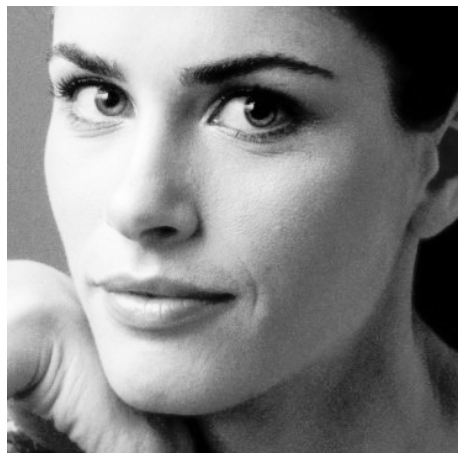
\includegraphics[width=0.3\textwidth]{resources/Annotation_Correction/Fig_Intro/intro_0_0}
    \hfill
    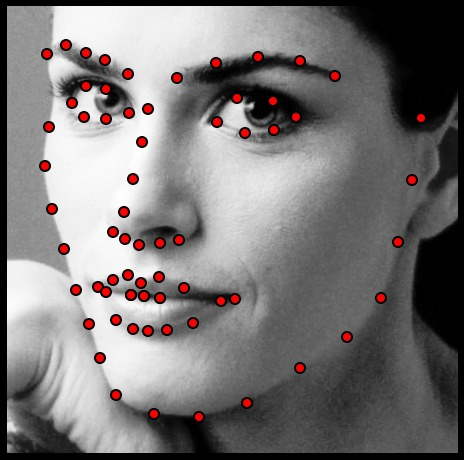
\includegraphics[width=0.3\textwidth]{resources/Annotation_Correction/Fig_Intro/intro_0_1}
    \hfill
    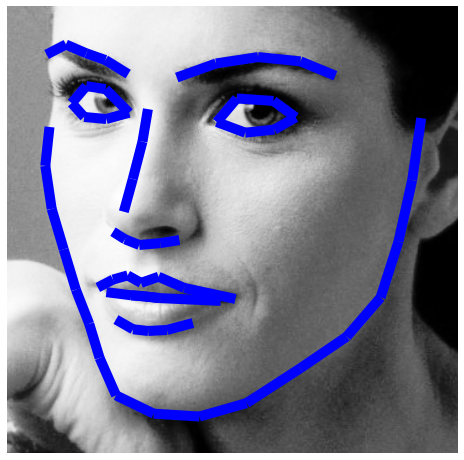
\includegraphics[width=0.3\textwidth]{resources/Annotation_Correction/Fig_Intro/intro_0_2}
    \\
    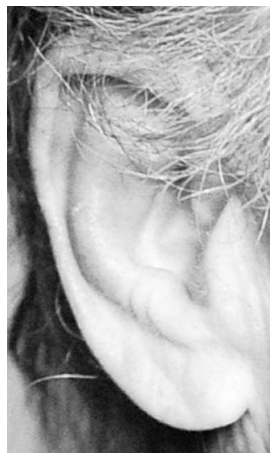
\includegraphics[width=0.15\textwidth]{resources/Annotation_Correction/Fig_Intro/intro_1_0}
    \hfill
    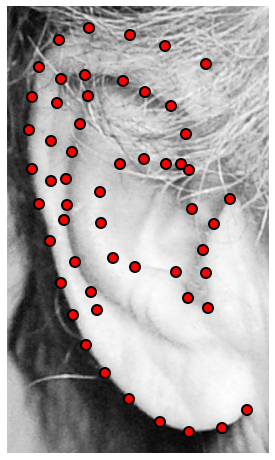
\includegraphics[width=0.15\textwidth]{resources/Annotation_Correction/Fig_Intro/intro_1_1}
    \hfill
    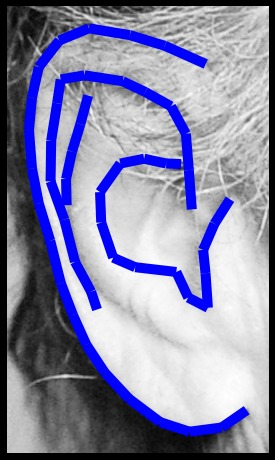
\includegraphics[width=0.15\textwidth]{resources/Annotation_Correction/Fig_Intro/intro_1_2}
    \hfill
    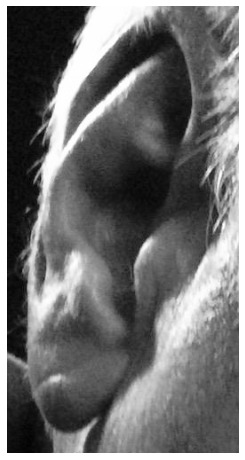
\includegraphics[width=0.15\textwidth]{resources/Annotation_Correction/Fig_Intro/intro_1_3}
    \hfill
    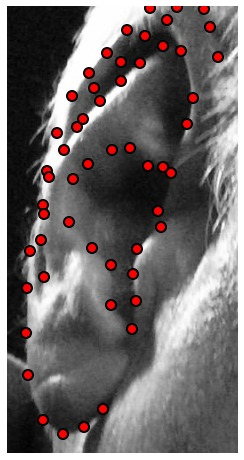
\includegraphics[width=0.15\textwidth]{resources/Annotation_Correction/Fig_Intro/intro_1_4}
    \hfill
    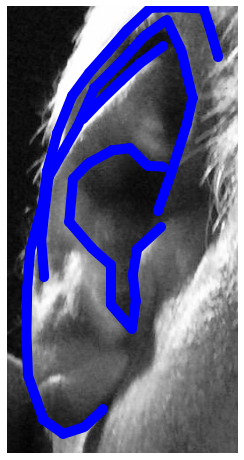
\includegraphics[width=0.15\textwidth]{resources/Annotation_Correction/Fig_Intro/intro_1_5}
    \\
    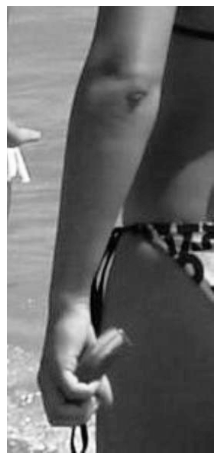
\includegraphics[width=0.15\textwidth]{resources/Annotation_Correction/Fig_Intro/intro_2_0}
    \hfill
    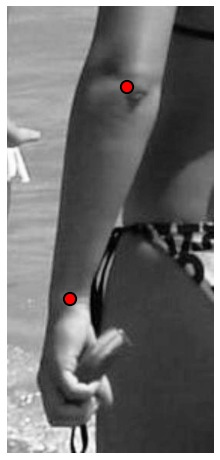
\includegraphics[width=0.15\textwidth]{resources/Annotation_Correction/Fig_Intro/intro_2_1}
    \hfill
    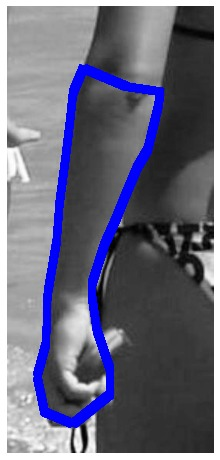
\includegraphics[width=0.15\textwidth]{resources/Annotation_Correction/Fig_Intro/intro_2_2}
    \hfill
    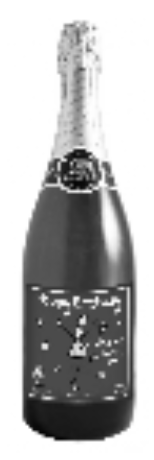
\includegraphics[width=0.15\textwidth]{resources/Annotation_Correction/Fig_Intro/intro_2_3}
    \hfill
    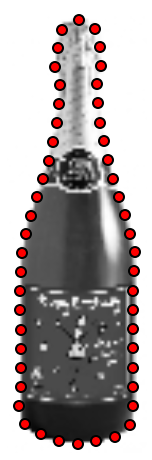
\includegraphics[width=0.15\textwidth]{resources/Annotation_Correction/Fig_Intro/intro_2_4}
    \hfill
    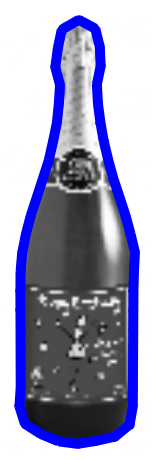
\includegraphics[width=0.15\textwidth]{resources/Annotation_Correction/Fig_Intro/intro_2_5}
    \\
    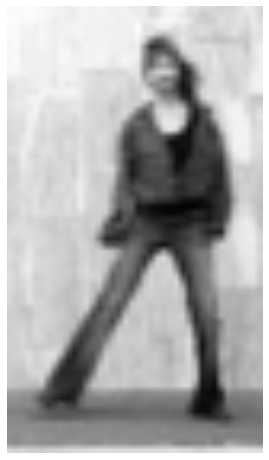
\includegraphics[width=0.15\textwidth]{resources/Annotation_Correction/Fig_Intro/intro_3_0}
    \hfill
    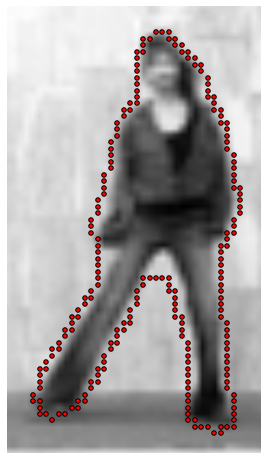
\includegraphics[width=0.15\textwidth]{resources/Annotation_Correction/Fig_Intro/intro_3_1}
    \hfill
    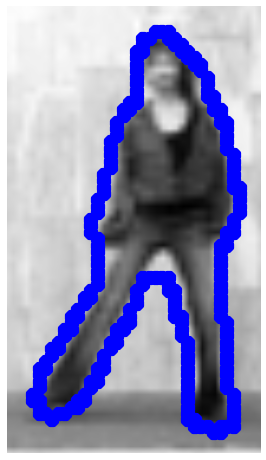
\includegraphics[width=0.15\textwidth]{resources/Annotation_Correction/Fig_Intro/intro_3_2}
    \hfill
    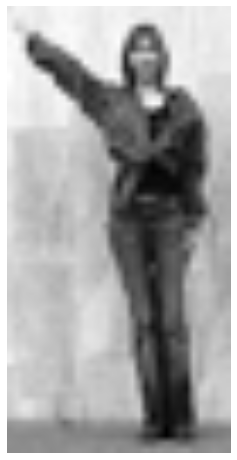
\includegraphics[width=0.15\textwidth]{resources/Annotation_Correction/Fig_Intro/intro_3_3}
    \hfill
    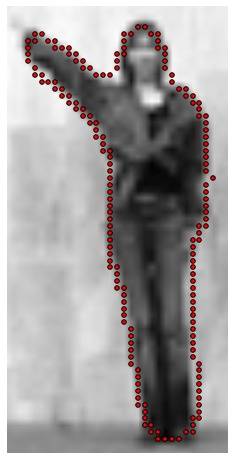
\includegraphics[width=0.15\textwidth]{resources/Annotation_Correction/Fig_Intro/intro_3_4}
    \hfill
    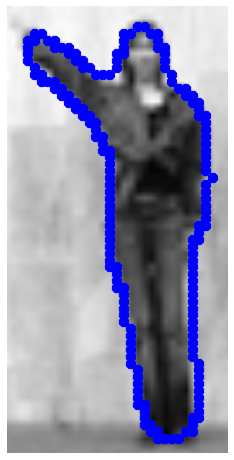
\includegraphics[width=0.15\textwidth]{resources/Annotation_Correction/Fig_Intro/intro_3_5}
    \caption{Demonstration of classical landmark annotation and curve annotation of faces, ears, bottles and human actions.}
    \label{fig:intro}
\end{figure}

Building and fitting statistical deformable models (SDMs) of objects is a well-studied and popular area in the intersection of computer vision and machine learning~\cite{Cootes1995, Cootes2001, Matthews2004, Saragih2011, Belhumeur2011, Zhu2012, Xiong2013}, where SDMs have been widely applied on object detection, part localisation, model reconstruction, fitting, recognition and tracking using manual annotated data. In recent past, We have witnessed tremendous developments in building and fitting models of human face and body using images captured in unconstrained recording conditions, usually referred to as ``in-the-wild"~\cite{Belhumeur2011, Cao2012, Zhu2012, Xiong2013, Asthana2013, Tzimiropoulos2014, Asthana2014}. This is attributed to: 
\begin{itemize}

\item The abundance of complex visual data, spread mostly through the internet via web services such as Youtube, Flickr and Google Images. The latter has led to the development of large databases of ``in-the-wild" images of human faces and bodies~\cite{Belhumeur2011, Le2012, Zhu2012, Burgos2013}. Equally important is the task of manual annotation of images with regards to face and body parts and that has been undertaken by several research teams~\cite{sagonas_iccv_300w_2013}.

\item The development of powerful visual features, able to describe objects and its parts in a robust manner (e.g., Scale Invariant Feature Transforms (SIFT)~\cite{lowe1999object}, Histogram of Oriented Gradients (HoGs)~\cite{Dalal2005} and recently Deep Convolutional Neural Networks~\cite{sermanet2013overfeat}), as well as generative and discriminative methodologies for learning deformable models. 

\end{itemize}

Nevertheless, there are two drawbacks on building deformable models that rely on landmarks: 
\begin{itemize}

\item Annotating with regards to consistent landmark annotation is extremely time consuming, tedious and labour intensive work~\cite{sagonas_iccv_300w_2013}, which usually can be performed by a trained person. Furthermore, for many objects it requires a highly skilled person to identify and annotate a set of images with regards to a consistent set of landmarks. For example human ears have very complicated inner structures (e.g. helix, crus antihelicis, scapha, tragus, lobe etc.) which differs remarkably between ears. Moreover, certain ear parts, such as  Fossa Triangularies and Crus Helicis, do not appear in all ears and  their visibility is highly sensitive to pose and illumination variation. Figure \ref{fig:formal_ear} demonstrated major feature components of a standard ear~\cite{Pflug2012}. 

\begin{figure}[ht]
    \centering
    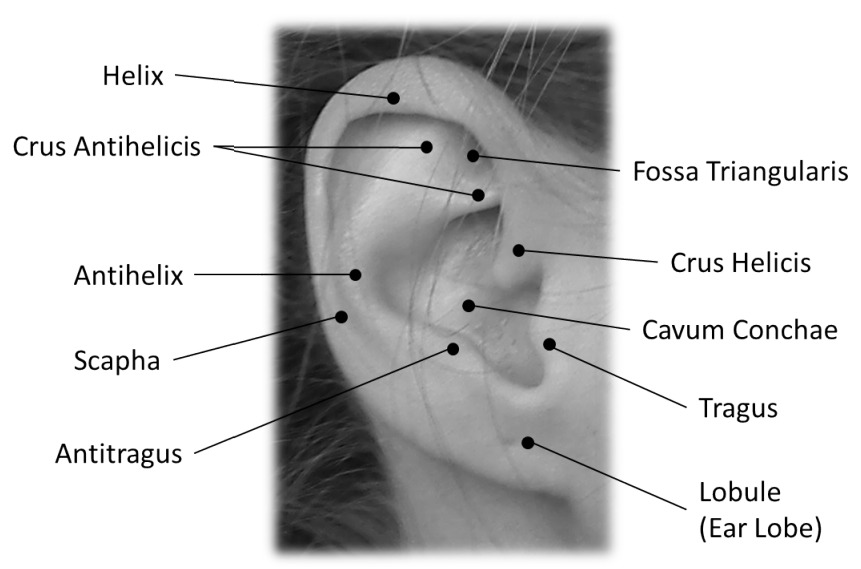
\includegraphics[width=0.5\textwidth]{resources/Background/formal_ear} 
    \caption{Ear with Clear Features}
    \label{fig:formal_ear}
\end{figure}

\begin{figure}[ht]
    \centering
    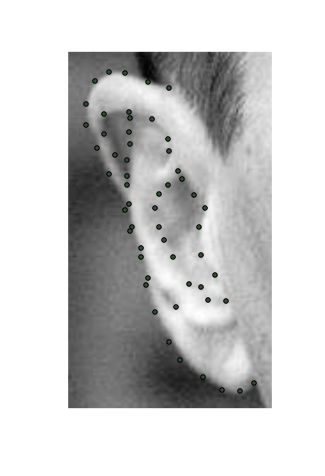
\includegraphics[width=0.22\textwidth]{resources/Background/hidden_feature_ear} 
    \hfill
    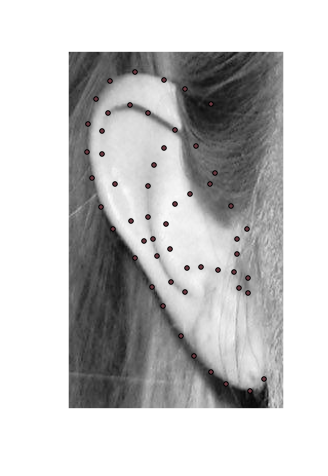
\includegraphics[width=0.22\textwidth]{resources/Background/hidden_feature_ear2} 
    \hfill
    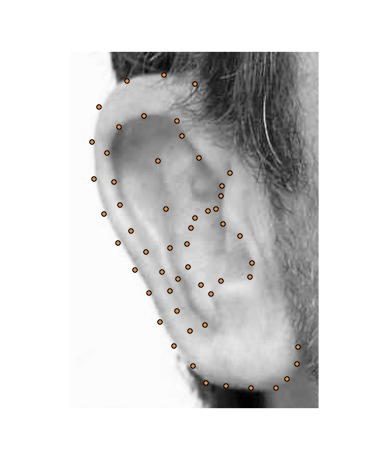
\includegraphics[width=0.22\textwidth]{resources/Background/hidden_feature_ear3} 
    \hfill
    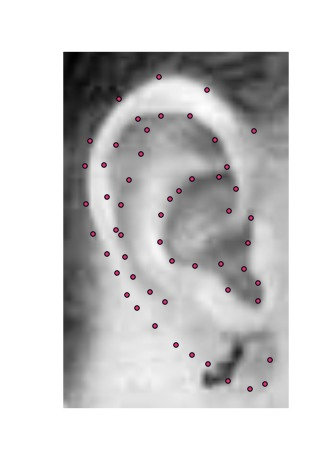
\includegraphics[width=0.22\textwidth]{resources/Background/hidden_feature_ear4} 
    \caption{Ears with Partial Features}
    \label{fig:hfe}
\end{figure}

But from Figure \ref{fig:hfe}, none of the shown ears has all features displayed clearly comparing to features of the standard ear. Some features are missing due to the pose variation or illumination (e.g. Figure \ref{fig:hfe1} has antihelix overlapped with helix) while some are because of the nature of ear, not all features exist on every ears (e.g. Figure \ref{fig:hfe2} has unclear crus antihelics, fossa triangularis and crus helicis are missing). The caption of each image in Figure \ref{fig:hfe} states the differences comparing to the standard ear.

\item The nature of many deformable objects does not allow them to be consistently annotated with regards to a set of landmarks (e.g. bottles, fruits etc.). Also the boundary/outline of objects, such as faces, ears, body can be very difficultly annotated consistently, Figure \ref{fig:intro}. That is why many state-of-the-art methods opt to leave the boundary out for comparison~\cite{Tzimiropoulos2014, Asthana2014}. The majority of the state-of-the-art methods for landmark-based deformable models~\cite{Cao2012, Zhu2012, Xiong2013, Tzimiropoulos2014, Asthana2014} are not applicable for objects with no consistent set of landmarks. 

\end{itemize}

To illustrate how time consuming careful annotation of ears is we lay down our own experience. A trained annotator needs an average of 4 minutes per image for the manual annotation of 55 landmarks. This means that the annotation of 1000 images requires a total of about 67 hours. 
Furthermore, training and fatigue largely influence the annotation accuracy. Hence, a second pass on the annotated data is, in many cases, necessary. Due to the fact that manual annotation is a rather costly and labour-intensive procedure, unsupervised learning of deformable models for the tasks of alignment has recently attracted some attention~\cite{kokkinos2007unsupervised,jojic2006escaping,jiang2009learning,liu2009simultaneous,baker2004automatic,cox2008least,cootes2004groupwise,frey2003learning}. Nevertheless, the method of~\cite{antonakos2014automatic} requires a consistent set of shapes annotated with landmarks to perform deformable face congealing. Finally, since the problem of fully unsupervised discovery of the deformations of arbitrary objects is a very difficult and ill-posed problems the limited number of methods that have been applied for the task cannot be applied for arbitrary collection of images collected ``in-the-wild". 

% TODO: Diffeomorphic Registration
Researches~\cite{cootes2004groupwise,cootes2004diffeomorphic,cootes2010computing,rueckert2006diffeomorphic,rueckert1999nonrigid,koelstra2010dynamic} also introduced methods for diffeomorphic image/shape registration, which put shapes in dense correspondence. Transformations between pairwise/groupwise images are diffeomorphic. Diffeomorphic deformations are smooth and invertible that, to be more specific, every points in shape $A$ have one-to-one correspondence with points in shape $B$, and vise versa. However, researches have shown there is no gaurentee that diffeomorphic algorithms can outperform algorithms with no diffeomorphism\cite{crum2004framework}.

We provide a solution for annotating an object with regards to its deformations that requires considerable less effort and in the same time can be used to define statistical deformations for objects without consistent set of landmarks. That is, we argue that it is better to annotate an object with regards to a set of continues lines that describe the shape of the object. An example is provided in Figure \ref{fig:intro} where the shape of the facial parts is annotated with continuous lines instead of a number of discrete landmarks. Similarly, the shape annotations for the ear, a bottle and human body is shown in Figure \ref{fig:intro} Annotating facial images by following this procedure takes less than 30 secs per image. Furthermore, these shapes can be automatically produced by recent methods that perform discriminative segmentation of objects. 

Furthermore, we show that flow methods have mature enough so that it can be used to densely annotate the proposed shapes using simple, as well as more recent and robust shape representations methods~\cite{Garg2013,Nguyen2013}.  In particular, to build dense correspondence between independent shapes, we apply optical flow on shapes with low rank constrains, so we name it shape flow. Optical flow is originally applied to video sequences that several assumptions holds, illumination consistency and motion smoothness, while shapes having no motion smoothness completely as all training data are independent. Low rank constrain plays important role to simulate motion smoothness assumption. 

We show that this way dense correspondences between images can be established and dense Active Appearance Models (AAMs) can be build on top of that. We show that the proposed methodology even though not tailored to landmark localization can be applied for landmark localization achieving very good performance. Finally, we demonstrate the performance of the proposed methodology for describing objects that do not have consistent landmarks. To the best of our knowledge this is the first methodology which can create a dense statistical model for AAM which can operate in ``in-the-wild".

Summarizing, the contributions proposed in this report are:
\begin{itemize}
  \item Constructing SDMs using training data with inconsistent annotation.
  \item Introduce highly effective curve annotation which tremendously reduces manual work overload but maintains same performance level against state-of-the-art SDMs.
  \item Building dense correspondent SDMs with shape flow
\end{itemize}


\section{Publications}
A list of publications are provided in this section. All publications were authored during the course of this Ph.D. thesis. There are two sections of publications: 1) publications that are directly related to the contents of this thesis (Section~\ref{label:related_pubs}) and 2) publications that are relatively relevant (Section~\ref{label:other_pubs}).

\subsection{Related Publications}
\label{label:related_pubs}

\begin{itemize}
  \item Ear Journal (TODO: To be complete)
  \item IJCV DenseReg and Pose Journal
  \item FG2018 Dense Pose
  \item FG2017 Ear Deformable Models
  \item CVPR2016: Annotation Correction
\end{itemize}

\subsection{Other Publications}
\label{label:other_pubs}

\begin{itemize}
  \item DeepMind \& Brain Project: publication somewhere (could be NIPS)
  \item UVGAN
  \item Joint Multi-view Face Alignment in the Wild
  \item Marginal Loss for Deep Face Recognition
  \item Semi-autonomous Data Enrichment Based on Cross-task Labelling of Missing Targets for Holistic Speech Analysis
\end{itemize}

\subsection{Outline}


